\section{Requirement Document}\label{sec:requirement-document}
\begin{figure}[H]
    \centering
    \caption[]{Requirement Document (Page 1)}
    \label{fig:requirement-document-1}
    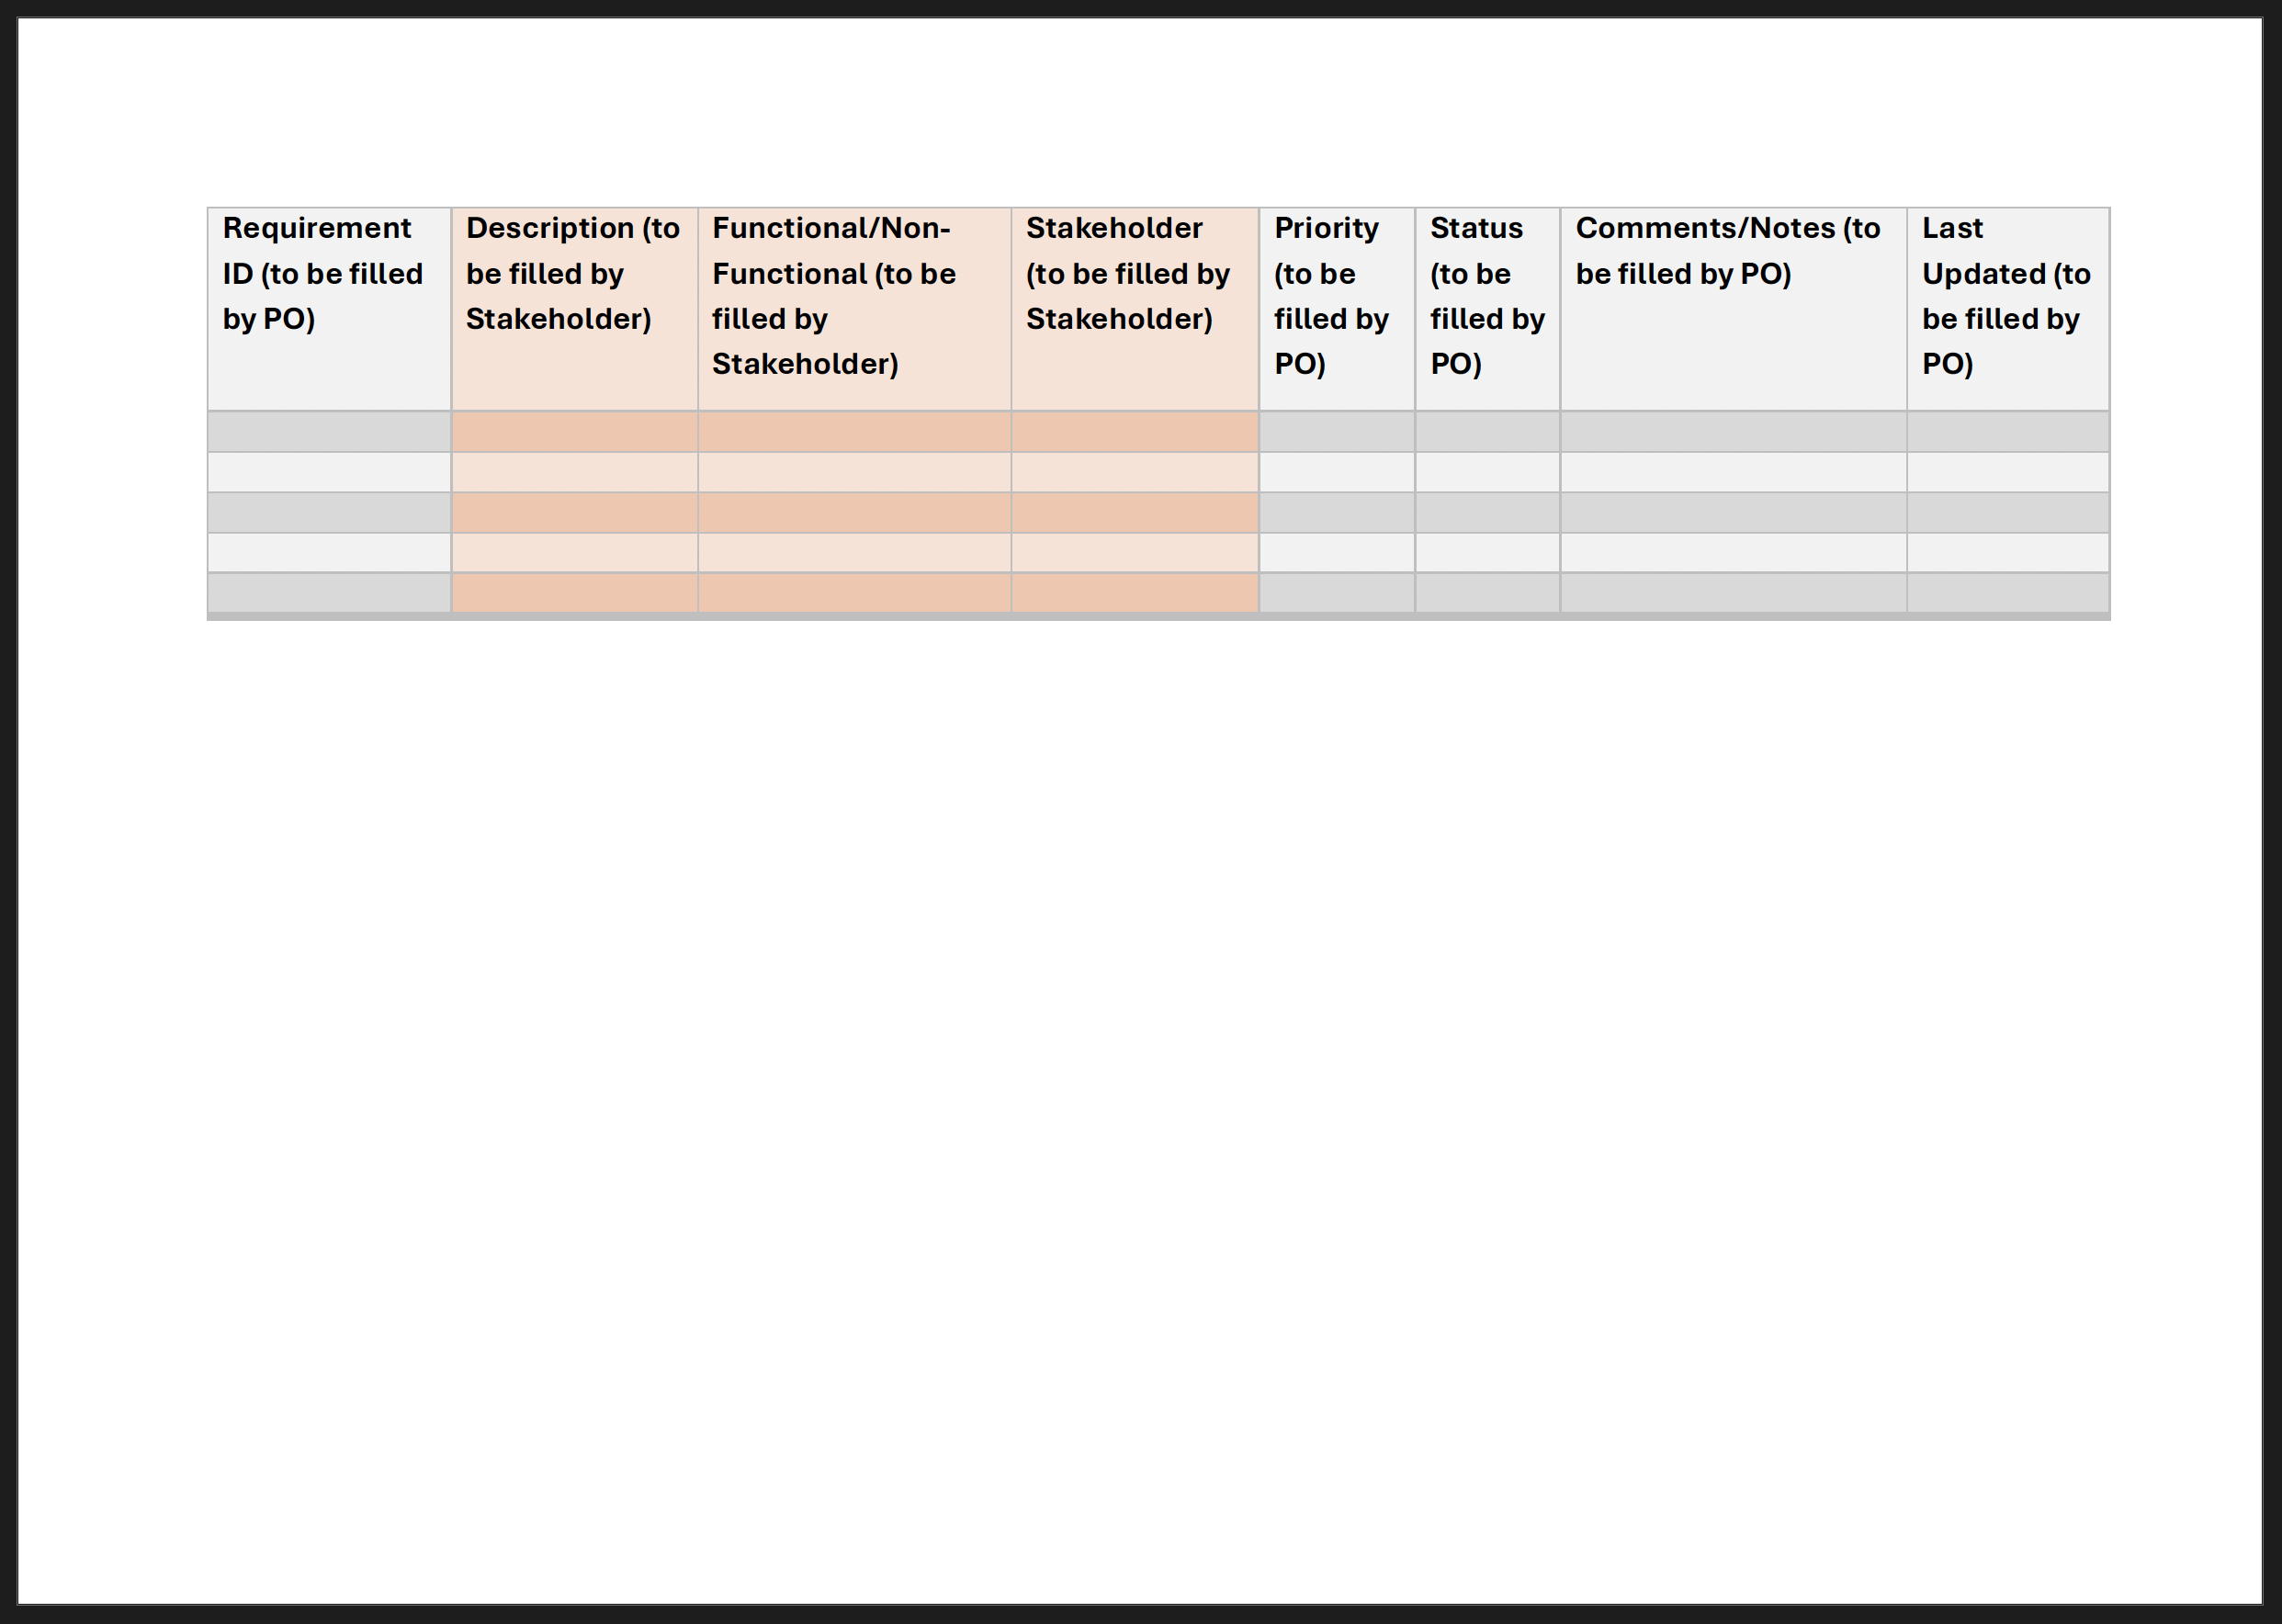
\includegraphics[width=1\textwidth]{abbildungen/RE/Word/RequirementDocument1}
\end{figure}
\begin{figure}[H]
    \centering
    \caption[]{Requirement Document (Page 2)}
    \label{fig:requirement-document-2}
    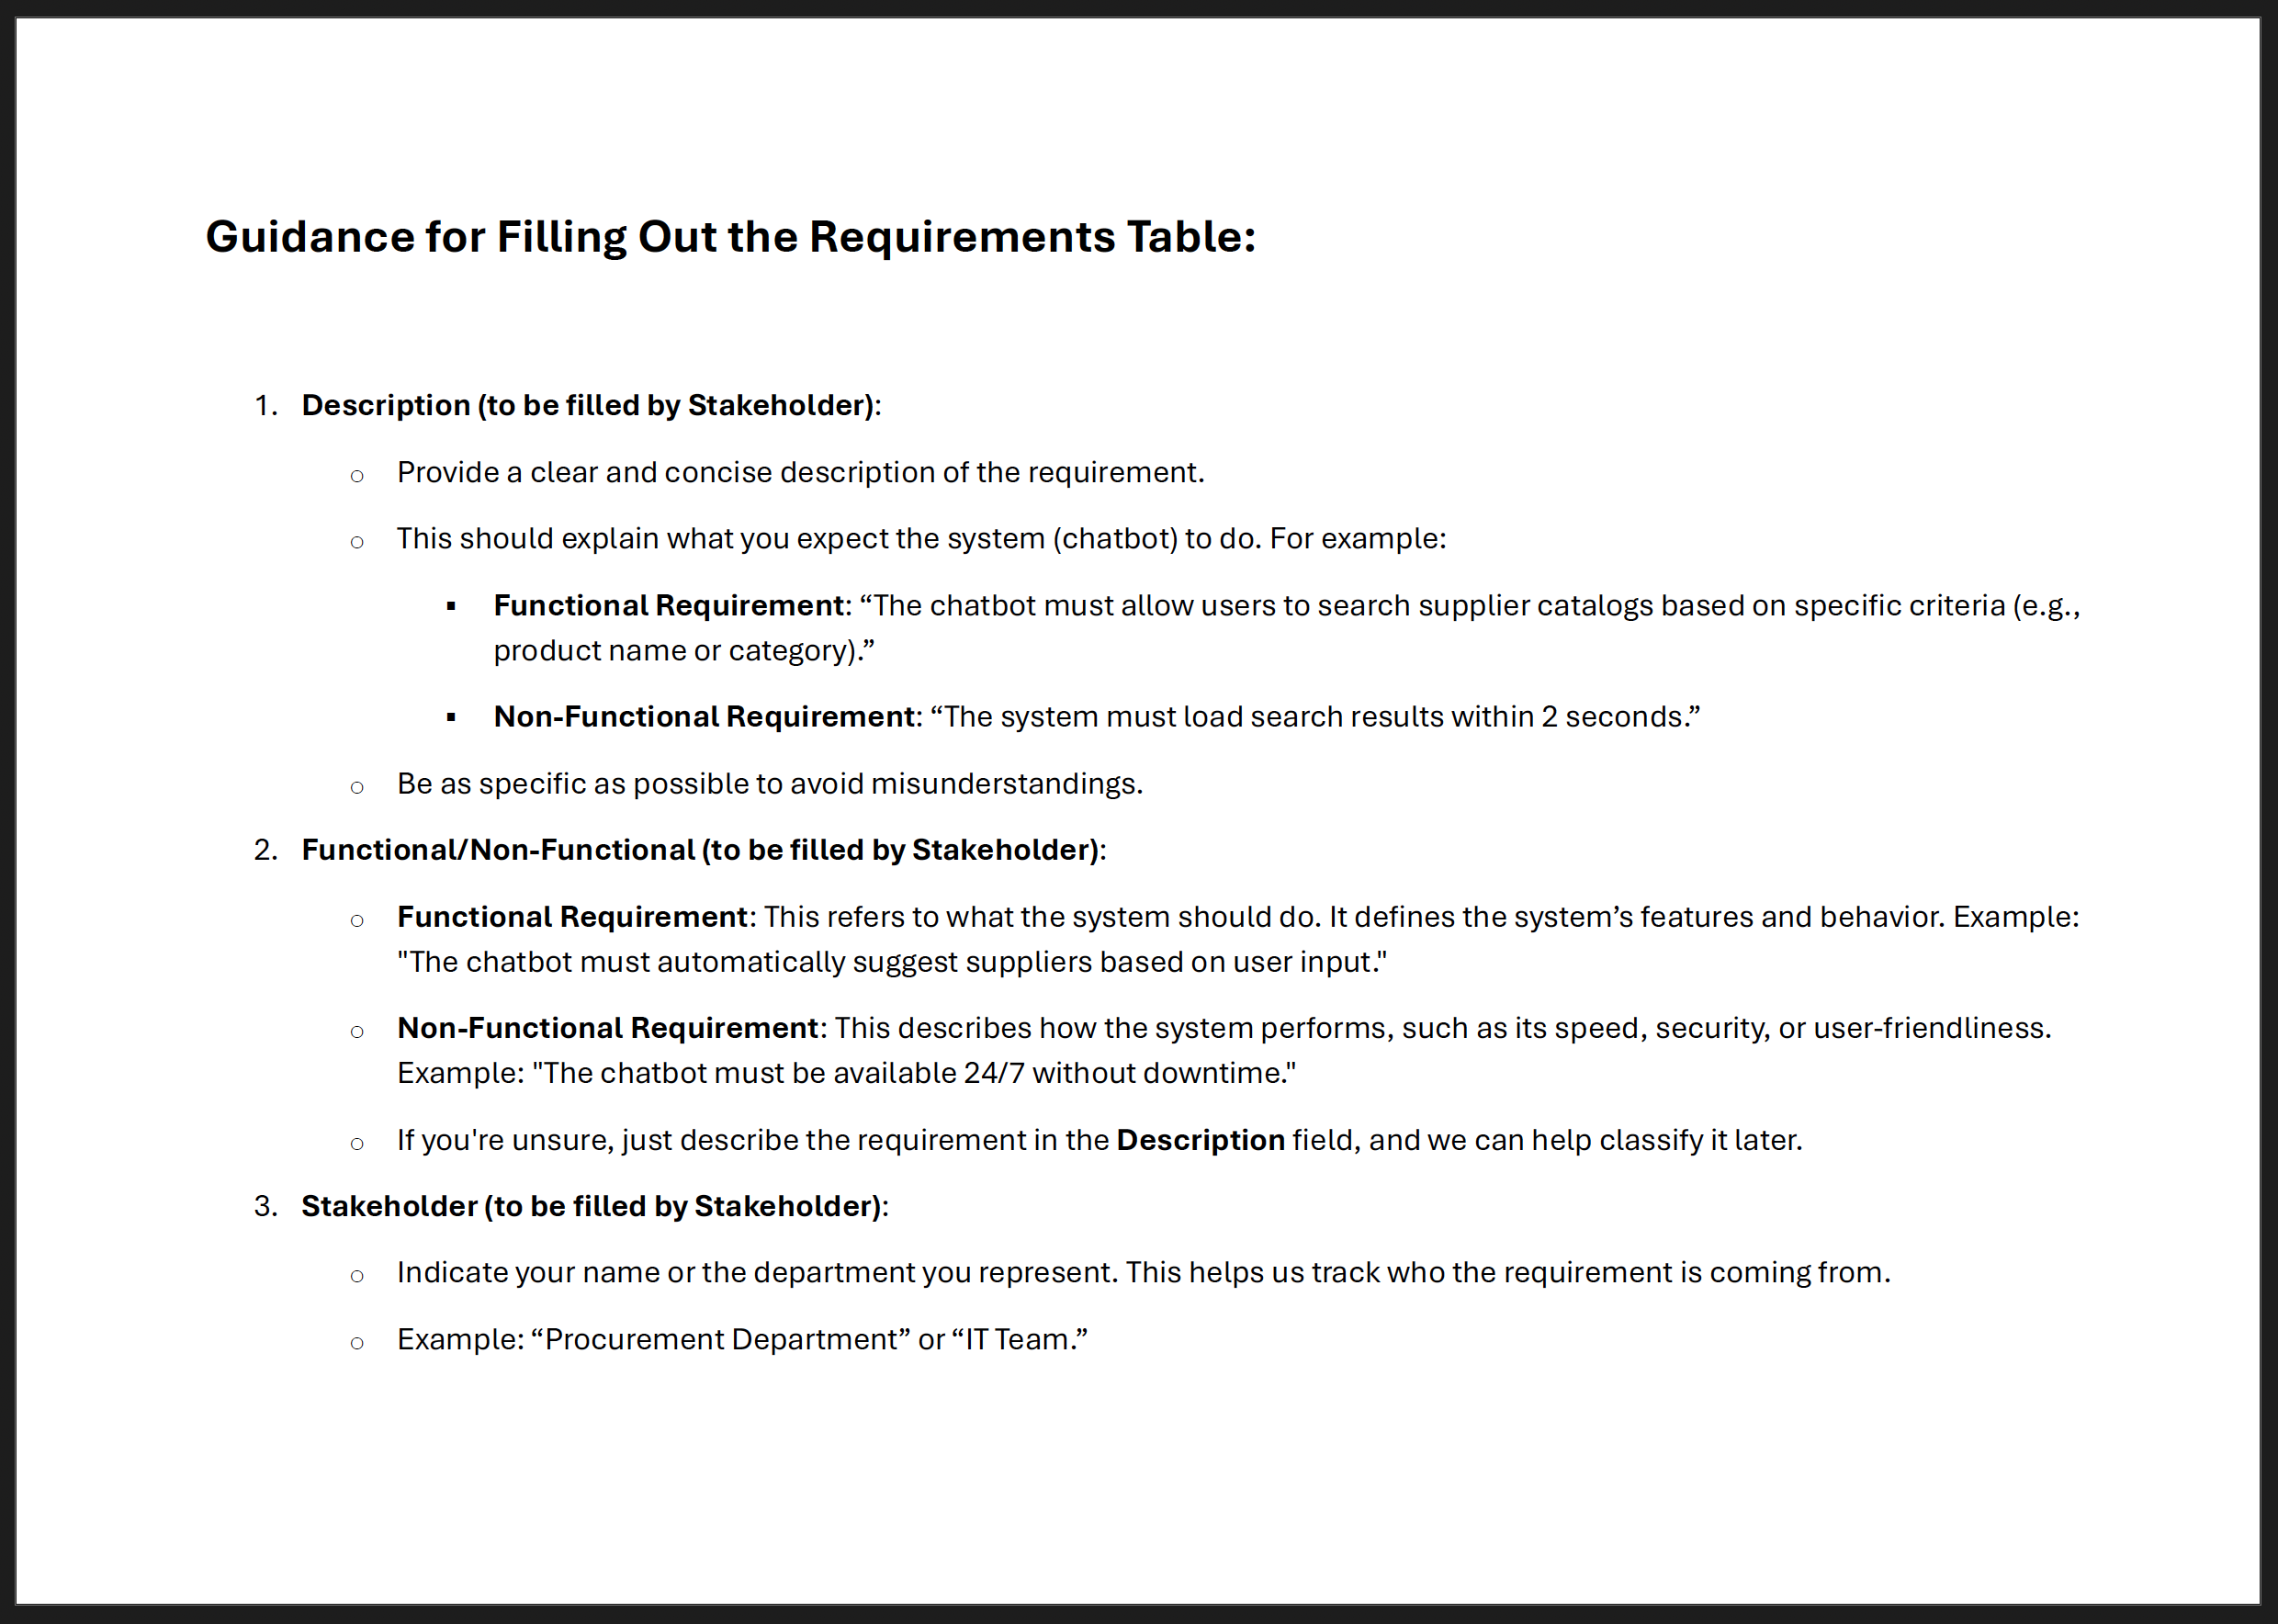
\includegraphics[width=1\textwidth]{abbildungen/RE/Word/RequirementDocument2}
\end{figure}

\section{Requirement Elicitation}\label{sec:requirement-elicitation}
\subsection{Screen Mock-Ups in Miro}\label{subsec:screen-mock-ups-in-miro}
\subsection{Screen Prototypes in Figma}\label{subsec:screen-prototypes-in-figma}
\subsection{Filled-out Requirement Documents}\label{subsec:filled-out-requirement-documents}